\documentclass[conference]{IEEEtran}

\ifCLASSINFOpdf
\else
\fi

\hyphenation{op-tical net-works semi-conduc-tor}

%% packages
% graph
\usepackage{graphicx}
\usepackage{epstopdf}
\usepackage{array}
\usepackage{rotating}
\usepackage{tabularx}
% math
\usepackage{amsfonts}
\usepackage{mathtools}
% algorithm
\usepackage{algorithm,algorithmic}% http://ctan.org/pkg/algorithms


\begin{document}


\title{A Distributed and Tensor-based Approach for Multidimensional Dictionary Learning}


% author names and affiliations
% use a multiple column layout for up to three different
% affiliations
\author{\IEEEauthorblockN{Thiago P de B Vieira}
\IEEEauthorblockA{
	Department of Electrical Engineering\\
	University of Brasilia\\
	Bras\'ilia-DF, Brazil\\
	Emai	l: tpbvieira@gmail.com
}

\and

\IEEEauthorblockN{Andr\'e L. F. de Almeida}
\IEEEauthorblockA{
	Department of Teleinformatics Engineering\\
	Federal University of Cear\'a\\
	Fortaleza, Brazil\\
	Emai	l: andre.almeida@ieee.org
}

\and

\IEEEauthorblockN{Florian Roemer\\ and Jo\~ao Paulo C. L. da Costa}
\IEEEauthorblockA{
	Institute for Information Technology\\
	Ilmenau University of Technology\\
	Ilmenau, Germany
}

}


\maketitle


\begin{abstract}
The abstract goes here.
\end{abstract}

\IEEEpeerreviewmaketitle

\section{Introduction}

Dictionary Learning is a signal processing technique for sparse representation of signals as basis vectors, learning the representations from training data, as dictionaries. The sparse representation in terms of such dictionaries has attracted increased interest for compressive sensing and for solving problems such as denoising, compression, classification, data decomposition, feature extraction and image processing \cite{tosic2011dictionary, zhang2010discriminative, zhu2016coupled,ravishankar2011mr}.

In some applications the data and its dictionary are multidimensional, e.g., when estimating jointly behavior of users in social networks. Computing tensor decompositions of multi-way datasets is particularly useful to extract hidden patterns and structure in multidimensional data analytics problems \cite{kolda2009tensor}. Tensor-based algorithms for dictionary learning can improve the performance for cases of multidimensional and separable data, regarding the dictionary identification rating, the required number of training samples and iterations for the optimization problem \cite{roemer2014tensor}. 

Multidimensional parameter estimation and learning multidimensional separable dictionaries are growing research problems. Roemer \emph{et al.} \cite{roemer2014tensor} show that the multidimensional dictionary estimation problem can be efficiently formulated in terms of tensors, and that their results outperform existing schemes by exploiting the multilinear structure of the problem.

Existing dictionary learning schemes can be applied to multidimensional analysis and obtain valuable results. However, the performance of tensor-based algorithms outperform existing schemes when dealing with growing multidimensional datasets, as can be seen in Figures \ref{fig:fig1} and \ref{fig:fig2}, which show that the detection rating of traditional algorithms decreases over the dataset increasing.

\begin{figure}[!htb]
     \centering 
	 \includegraphics[width=0.4\textwidth]{figures/5_20_2000_1000_100.eps}
     \caption{Matrix of 1.000 elements, 2000 sample training, 100 iterations}
     \label{fig:fig1}
\end{figure}

\begin{figure}[!htb]
     \centering 
	 \includegraphics[width=0.4\textwidth]{figures/5_20_2000_24000_100.eps}
     \caption{Matrix of 24.000 elements, 2000 sample training, 100 iterations}
     \label{fig:fig2}
\end{figure}

Figures \ref{fig:fig1} and \ref{fig:fig2} show the evaluation of tensor-based and traditional dictionary learning algorithms for dictionary reconstruction of a multidimensional and separable data. Figure \ref{fig:fig1} presents the results for dictionary reconstruction from a matrix of 1000 elements, while Figures \ref{fig:fig2} presents the results from a matrix with 24000 entries. It is possible to observe better detection rating for tensor-based algorithms. However, tensor-based algorithms face challenges to achieve reasonable processing time to handle large-scale tensor factorizations \cite{de2014distributed}, demanding efforts in order to explore distributed processing techniques for tensor-based analytics of large datasets.

We propose a distributed and tensor-based approach for multidimensional dictionary learning in order to obtain better processing time for larger datasets. We focus on a distributed implementation of T-MOD \cite{roemer2014tensor} algorithm, based on a modification of Almeida and Kibangou's \cite{de2014distributed} approach to use Tucker-2 decomposition. We perform experiments to test different methods for learning dictionaries, evaluating the processing time and the reconstruction of a dictionary of multidimensional and separable data.

\section{Data Model}

Consider a generic sparse recovery problem of the following form

\begin{equation}\label{eq:eq01}
\boldsymbol{X} = \boldsymbol{A} \cdot \boldsymbol{S} + \boldsymbol{W},
\end{equation}

where $\boldsymbol{X} \in \mathbb{C}^{M \times T}$ represents $T$ consecutive observations from $M$ features, $\boldsymbol{A} \in \mathbb{C}^{M \times N}$ is the overcomplete dictionary, $\boldsymbol{S} \in \mathbb{•}hbb{C}^{N \times T}$ represents the sparse coefficient matrix, $\boldsymbol{W} \in \mathbb{C}^{M \times T}$ is the additive noise, and $M < N < T$.

Consider a sparse recovery problem for a separable 2-D manifold, i.e., a manifold that can be written as the product of two 1-D manifolds. If we choose a separable 2-D sampling grid, we can write the 2D sparse recovery problem as

\begin{equation}\label{eq:eq02}
\boldsymbol{X} = (\boldsymbol{A}^{(1)} \otimes \boldsymbol{A}^{(2)}) \cdot \boldsymbol{S} + \boldsymbol{W},
\end{equation}

where $\boldsymbol{A} = (\boldsymbol{A}^{(1)} \otimes \boldsymbol{A}^{(2)})$, $\boldsymbol{A}^{(1)} \in \mathbb{C}^{M_1 \times N_1}$, $\boldsymbol{A}^{(2)} \in \mathbb{C}^{M_2 \times N_2}$, $M = M_1 \times M_2$, and $N = N_1 \times N_2$.

The Kronecker model (\ref{eq:eq02}) can be rewritten in an equivalent tensor form. Applying the algebraic rules for unfoldings of n-mode products \cite{roemer2014tensor} we can rewrite (\ref{eq:eq02}) into a "Tucker-2" decomposition, as

\begin{equation}\label{eq:eq03}
\boldsymbol{\mathcal{X}} = \boldsymbol{\mathcal{S}} \times_1 \boldsymbol{A}^{(1)} \times_2 \boldsymbol{A}^{(2)} +  \boldsymbol{\mathcal{W}},
\end{equation}

where $\boldsymbol{\mathcal{X}} \in \mathbb{C}^{M_1 \times M_2 \times T}$, $\boldsymbol{\mathcal{S}} \in \mathbb{C}^{N_1 \times N_2 \times T}$, and $\boldsymbol{\mathcal{W}} \in \mathbb{C}^{M_1 \times M_2 \times T}$ are rearranged versions of the matrices $\boldsymbol{X}$, $\boldsymbol{S}$, and $\boldsymbol{W}$ such that $\boldsymbol{X} = [\boldsymbol{\mathcal{X}}]_{(3)}^T$, $\boldsymbol{S} = [\boldsymbol{\mathcal{S}}]_{(3)}^T$, and $\boldsymbol{W} = [\boldsymbol{\mathcal{W}}]_{(3)}^T$, respectively.

We consider a randomly generated data in order to evaluate the proposed approach, where initially $\boldsymbol{A}^{(1)}$ and $\boldsymbol{A}^{(2)}$ are gaussian distributed and randomly generated, then the dictionary $\boldsymbol{A}$ is obtained. In order to be able to evaluate the dictionary reconstruction, the sparse data $\boldsymbol{\mathcal{X}}$ is generated from the dictionary $\boldsymbol{A}$, which is used for further comparisons. We adopt 20 as the signal-to-noise ratio (snr) and 5 as the sparseness factor of the data $\boldsymbol{\mathcal{X}}$. 

The dictionary estimation is evaluated by applying the proposed approach to estimate the dictionary $\boldsymbol{A}$ from the sparse data $\boldsymbol{\mathcal{X}}$, according the selected number of sample training and iterations for the optimization problem.

\section{Proposed Approach}

...

\section{Experiments}

...

\begin{figure}[!htb]
     \centering 
	 \includegraphics[width=0.4\textwidth]{figures/5_20_2000_4000_100.eps}
     \caption{Matrix of 4.000 elements, 2000 sample training, 100 iterations}
     \label{fig:facets_cross}
\end{figure}

\begin{figure}[!htb]
     \centering 
	 \includegraphics[width=0.4\textwidth]{figures/5_20_500_16000_100.eps}
     \caption{Matrix of 16.000 elements, 500 sample training, 100 iterations}
     \label{fig:facets_cross}
\end{figure}

\section{Conclusion}
The conclusion goes here.


\section*{Acknowledgment}
{\small This research was supported by ...}


\bibliographystyle{IEEEtran}
\bibliography{references}

\end{document}